\chapter{Membranes et transports membranaires}\label{ch:b1:membranes-transport}

Plongez un globule rouge dans de l'eau pure~: il gonfle et éclate en une
seconde~; plongez-le dans une saumure~: il se ratatine. Remettez-le dans
du \omterm{def:b1:mammal-organization:compartments}{plasma}~: il garde sa forme biconcave quatre mois durant, en expulsant
du sodium et en captant du potassium à chaque seconde de ce temps. La
membrane qui fait cela est épaisse de cinq nanomètres --- un film de
lipides de deux molécules d'épaisseur, traversé de protéines --- et
c'est la limite à travers laquelle se réalise finalement chacun des
échanges du \cref{ch:b1:organism-environment}. Ce chapitre décrit la
structure de la membrane, la physique de ce qui la franchit sans aide,
les protéines qui transportent, pompent et canalisent le reste, le
potentiel électrique que ce trafic engendre, et les vésicules qui
déplacent ce qu'aucune protéine ne peut porter.

\section{La mosaïque fluide}

\begin{definition}[La membrane plasmique]\label{def:b1:membranes-transport:membrane}
La \emph{membrane plasmique}\index{membrane plasmique} --- comme toute
membrane de la \omterm{def:b1:cell-unit-of-life:cell}{cellule} --- est une \emph{bicouche
lipidique}\index{bicouche lipidique} d'environ \qty{5}{nm} d'épaisseur~:
deux feuillets de phospholipides (\cref{ch:b1:lipids}) dont les queues
hydrophobes se font face et dont les têtes polaires regardent les deux
milieux aqueux, avec du cholestérol entre les queues, et des
\emph{protéines membranaires}\index{proteine membranaire@protéine membranaire} enchâssées
dedans ou fixées dessus. Dans le modèle de la \emph{mosaïque
fluide}\index{modele de la mosaique fluide@modèle de la mosaïque fluide} (Singer et Nicolson, 1972),
la bicouche est un fluide bidimensionnel dans lequel lipides et
protéines diffusent latéralement, et les protéines forment une mosaïque
d'unités indépendantes, non un revêtement continu. Les deux faces
diffèrent~: les sucres fixés aux lipides et aux protéines ne regardent
que vers l'extérieur (le \emph{glycocalyx}), et certains phospholipides
sont confinés à un seul feuillet.
\end{definition}

\begin{omfigure}
\begin{tikzpicture}[font=\footnotesize, line cap=round]
  % bilayer: heads as circles, tails as lines
  \foreach \i in {0,...,21} {
    \pgfmathsetmacro{\x}{0.42*\i}
    \fill[omDef!60] (\x,1.35) circle (0.16);
    \draw[omDef!70!black, thick] (\x-0.07,1.2) -- (\x-0.07,0.55) (\x+0.07,1.2) -- (\x+0.07,0.55);
    \fill[omDef!60] (\x,-0.35) circle (0.16);
    \draw[omDef!70!black, thick] (\x-0.07,-0.2) -- (\x-0.07,0.45) (\x+0.07,-0.2) -- (\x+0.07,0.45);
  }
  % cholesterol
  \foreach \x in {1.9,6.1,8.2} { \draw[omProp, very thick] (\x,1.1) -- (\x,0.6); \fill[omProp] (\x,1.15) circle (0.08); }
  % integral protein spanning (channel)
  \draw[thick, omThm!80!black, fill=omThm!30, rounded corners=3pt] (3.0,-0.7) rectangle (3.55,1.7);
  \draw[thick, omThm!80!black, fill=omThm!30, rounded corners=3pt] (3.85,-0.7) rectangle (4.4,1.7);
  \fill[white] (3.55,-0.6) rectangle (3.85,1.6);
  % integral protein (carrier)
  \draw[thick, omThm!80!black, fill=omThm!30, rounded corners=5pt] (6.8,-0.75) rectangle (7.7,1.75);
  % peripheral protein
  \draw[thick, omExo!80!black, fill=omExo!30] (5.3,1.75) ellipse (0.5 and 0.28);
  % glycocalyx sugar chains on outer face
  \foreach \x in {0.5,1.3,2.5,4.15,7.25,8.4} { \draw[omProp!80!black, thick] (\x,1.5) .. controls (\x+0.15,1.85) and (\x-0.15,2.1) .. (\x+0.1,2.4); \fill[omProp!70] (\x+0.1,2.45) circle (0.07); }
  % labels
  \node[anchor=east] at (-0.3,1.35) {têtes polaires};
  \node[anchor=east] at (-0.3,0.5) {queues hydrophobes};
  \node[anchor=east] at (-0.3,-0.35) {têtes polaires};
  \node[anchor=west, align=left] at (9.2,2.2) {chaînes de sucres~:\\ extérieur seul};
  \node[anchor=west, align=left] at (9.2,0.5) {\qty{5}{nm}};
  \node[anchor=north] at (3.7,-0.95) {protéine-canal};
  \node[anchor=north] at (7.25,-0.95) {transporteur};
  \node[anchor=south] at (5.3,2.6) {protéine extrinsèque};
  \node[anchor=north, omProp] at (1.5,-1.0) {cholestérol};
  \node[anchor=south east, gray] at (-0.3,2.4) {extérieur};
  \node[anchor=north east, gray] at (-0.3,-0.95) {cytosol};
  \draw[<->, gray] (9.05,1.35+0.16) -- (9.05,-0.35-0.16);
\end{tikzpicture}

{\small La \omterm{def:b1:membranes-transport:membrane}{mosaïque fluide}. Deux feuillets de phospholipides, queues
vers l'intérieur, avec du cholestérol parmi elles~; des \omterm{def:b1:membranes-transport:proteins}{protéines
intrinsèques} traversant la bicouche (un canal avec son pore, un
transporteur), une protéine extrinsèque sur une face, et des chaînes de
sucres sur la face externe seulement.}
\end{omfigure}

\begin{omfigure}
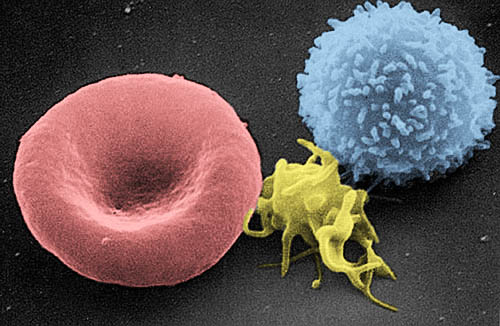
\includegraphics[width=0.4\linewidth]{images/book3/red-cells-nci.jpg}

{\small Un globule rouge, une plaquette et un lymphocyte au \omterm{prop:b1:cell-unit-of-life:microscopes}{microscope
électronique} à balayage (image colorisée). La forme biconcave du globule
rouge est tenue par un maillage protéique sous sa membrane~; il survit à
quatre mois de passages forcés dans des capillaires plus étroits que
lui. Image~: National Cancer Institute, domaine public.}
\end{omfigure}

\begin{proposition}[Les membranes sont des bicouches et des fluides]\label{prop:b1:membranes-transport:evidence}
La \omterm{def:b1:membranes-transport:membrane}{membrane plasmique} a exactement l'épaisseur de deux molécules de
lipides, et ses constituants se déplacent dans son plan.
\end{proposition}
\begin{proof}[Faits expérimentaux]
Gorter et Grendel (1925) extrayèrent les lipides d'un nombre connu de
globules rouges et les étalèrent en monocouche sur de l'eau~: l'aire
valait deux fois la surface totale des \omterm{def:b1:cell-unit-of-life:cell}{cellules}, donc la membrane est
une bicouche. La microscopie électronique montre toute membrane comme
deux lignes sombres (les têtes contrastées) encadrant un cœur pâle (les
queues), \qty{5}{nm} en tout. Frye et Edidin (1970) fusionnèrent une
\omterm{def:b1:cell-unit-of-life:cell}{cellule} de souris avec une \omterm{def:b1:cell-unit-of-life:cell}{cellule} humaine dont les protéines de surface
avaient été marquées par des colorants de deux couleurs~: après quarante
minutes à \qty{37}{\celsius}, les deux couleurs étaient complètement
mêlées sur toute la \omterm{def:b1:cell-unit-of-life:cell}{cellule} hybride, et pas du tout à \qty{4}{\celsius},
où le lipide est presque solide. Blanchir au laser une tache d'une
\omterm{def:b1:membranes-transport:membrane}{protéine membranaire} fluorescente et regarder la fluorescence revenir à
mesure que des molécules non blanchies y diffusent (FRAP) mesure la
diffusion latérale~: $\qty{1}{\micro m^2}$ en quelques secondes pour les
lipides, plus lentement pour les protéines, et nulle pour les protéines
ancrées au \omterm{def:b1:eukaryotic-cell:cytoskeleton}{cytosquelette}.
\end{proof}

\begin{definition}[Protéines membranaires]\label{def:b1:membranes-transport:proteins}
Les \omterm{def:b1:membranes-transport:membrane}{protéines membranaires}
\emph{intrinsèques}\index{proteine intrinseque@protéine intrinsèque} traversent la bicouche
par une ou plusieurs hélices hydrophobes et ne peuvent être extraites
qu'avec des détergents~; les protéines \emph{extrinsèques} sont fixées
sur une face. Par la fonction~: les \emph{transporteurs} (canaux,
transporteurs proprement dits, \omterm{def:b1:membranes-transport:transporters}{pompes}), les \emph{récepteurs} qui lient
un signal au-dehors et agissent au-dedans, les \emph{enzymes}, les
\emph{ancrages} reliant le \omterm{def:b1:eukaryotic-cell:cytoskeleton}{cytosquelette} à la \omterm{def:b1:body-plans-tissues:connective}{matrice extracellulaire},
et les protéines de \emph{reconnaissance} portant les sucres par
lesquels les \omterm{def:b1:cell-unit-of-life:cell}{cellules} s'identifient les unes les autres. Les protéines
font la moitié de la masse d'une membrane typique et presque toute sa
fonction.
\end{definition}

\section{Traverser la membrane sans aide}

\begin{proposition}[Perméabilité de la bicouche]\label{prop:b1:membranes-transport:permeability}
\index{permeabilite@perméabilité}
Une \omterm{def:b1:membranes-transport:membrane}{bicouche lipidique} pure est librement perméable aux petites
molécules apolaires ($\mathrm{O_2}$, $\mathrm{CO_2}$, $\mathrm{N_2}$,
stéroïdes), assez perméable aux petites molécules polaires non chargées
(eau, urée, éthanol), peu perméable aux molécules polaires plus grandes
(glucose, acides aminés), et pratiquement imperméable aux ions
($\mathrm{Na^+}$, $\mathrm{K^+}$, $\mathrm{Cl^-}$, $\mathrm{H^+}$) et
aux macromolécules. La perméabilité s'étend sur douze ordres de
grandeur, de $\qty{e-2}{cm/s}$ pour l'eau à $\qty{e-14}{cm/s}$ pour
$\mathrm{Na^+}$~: un cœur hydrophobe de \qty{3}{nm} d'épaisseur laisse
passer ce qui se dissout dans l'huile et arrête ce qui porte une charge.
\end{proposition}

\begin{theorem}[Loi de diffusion de Fick]\label{thm:b1:membranes-transport:fick}
\index{loi de Fick}\index{diffusion}
Le flux net $J$ d'un soluté à travers une membrane d'aire $S$ (en moles
par seconde) est proportionnel à la différence de concentration de part
et d'autre~:
\[
J = P\,S\,(c_{\text{ext}} - c_{\text{int}}),
\]
où le \emph{coefficient de perméabilité} $P$ (en \unit{m/s}) réunit le
coefficient de diffusion du soluté dans la membrane, sa solubilité dans
le lipide et l'épaisseur de la membrane ($P = DK/\ell$). La diffusion ne
demande pas d'énergie et descend toujours le gradient~; c'est un
\emph{transport passif}\index{transport passif}.
\end{theorem}
\begin{proof}
Dans la membrane, le soluté diffuse le long d'un profil de concentration
linéaire allant de $Kc_{\text{ext}}$ à $Kc_{\text{int}}$ ($K$ étant le
coefficient de partage entre lipide et eau)~; la première \omterm{thm:b1:membranes-transport:fick}{loi de Fick} en
milieu massif, $J/S = -D\,\dd c/\dd x$, donne $J/S = DK(c_{\text{ext}} -
c_{\text{int}})/\ell$.
\end{proof}

\begin{definition}[Osmose, potentiel hydrique]\label{def:b1:membranes-transport:osmosis}
L'\emph{osmose}\index{osmose} est la diffusion nette d'eau à travers une
membrane qui laisse passer l'eau mais non les solutés, de la solution où
l'eau est la plus concentrée (le moins de solutés) vers celle où elle
l'est le moins. Elle se décrit par le \emph{potentiel
hydrique}\index{potentiel hydrique} $\Psi$, le potentiel chimique de
l'eau exprimé comme une pression, nul pour l'eau pure à la pression
atmosphérique~:
\[
\Psi = \Psi_s + \Psi_p, \qquad \Psi_s = -RTc_s ,
\]
où $\Psi_s$, le \emph{potentiel osmotique}\index{potentiel osmotique},
diminue avec la concentration totale en solutés $c_s$ (en osmoles par
litre, loi de van 't Hoff) et $\Psi_p$, le \emph{potentiel de
pression}\index{potentiel de pression}, est la pression hydrostatique
au-dessus de l'atmosphérique. L'eau va toujours vers le $\Psi$ le plus
bas. À \qty{25}{\celsius}, $RT = \qty{2.48}{MPa.L/mol}$~: une solution à
\qty{0.3}{osmol/L} a $\Psi_s = \qty{-0.74}{MPa}$. Une solution est
\emph{isotonique}\index{isotonique} à une \omterm{def:b1:cell-unit-of-life:cell}{cellule} lorsqu'aucun flux net
d'eau n'a lieu, \emph{hypotonique} lorsque l'eau entre,
\emph{hypertonique} lorsqu'elle sort.
\end{definition}

\begin{omfigure}
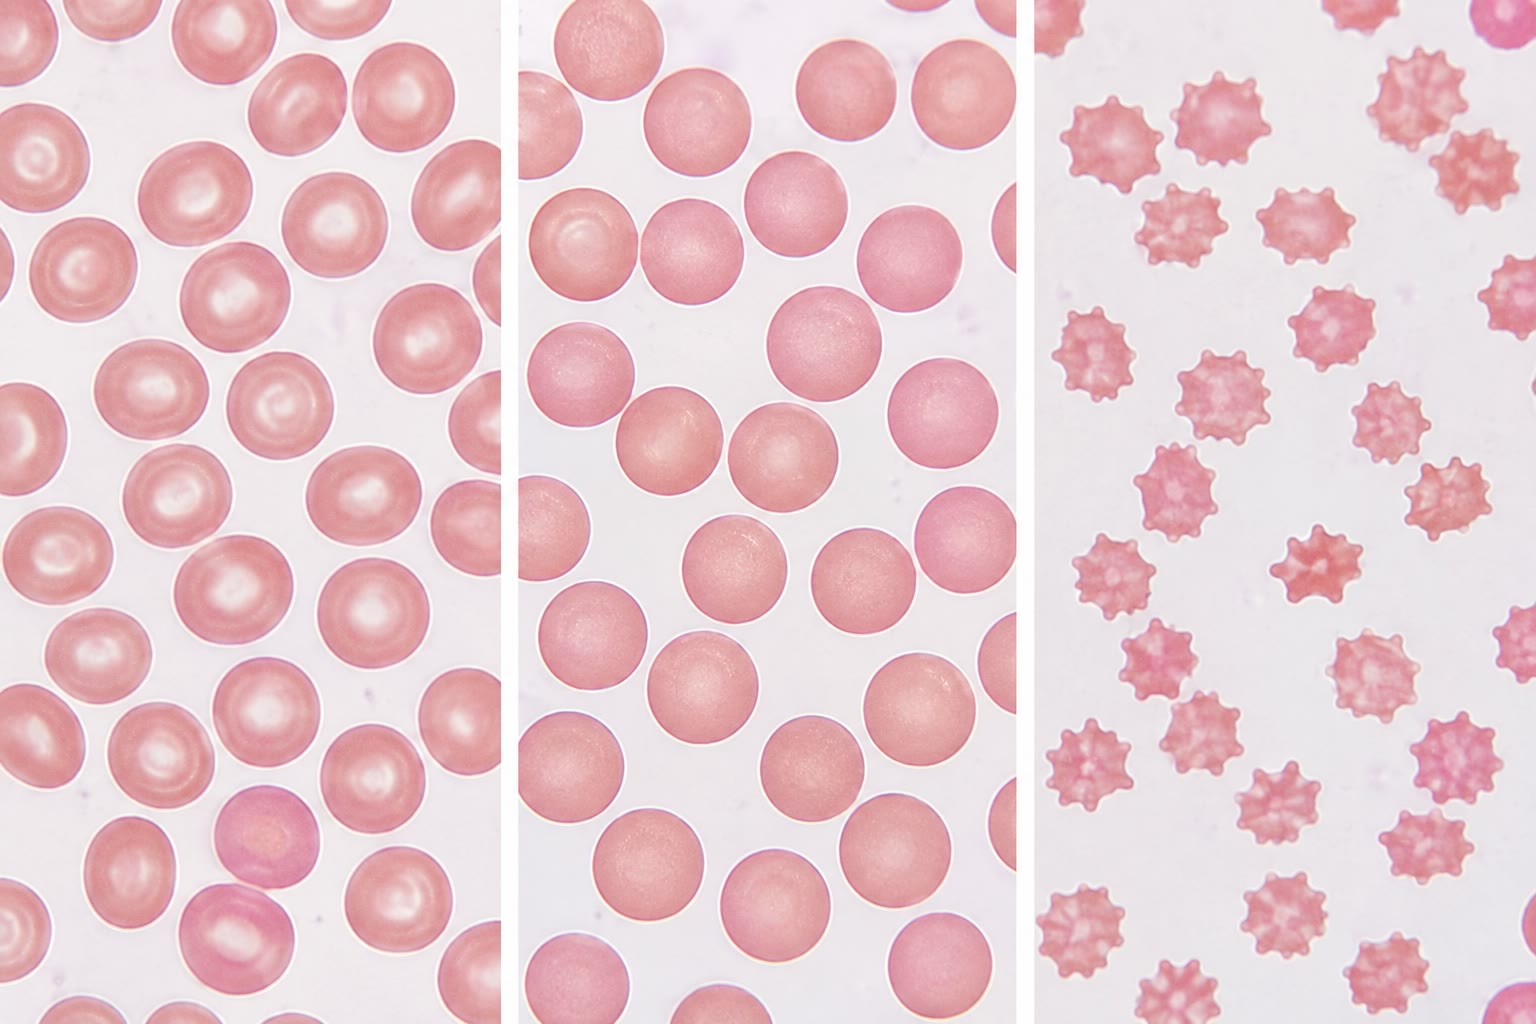
\includegraphics[width=0.78\linewidth]{images/book3/ai/b3-07-red-cells-osmosis.jpg}

{\small Des globules rouges dans une solution \omterm{def:b1:membranes-transport:osmosis}{isotonique} (disques
biconcaves), dans une solution hypotonique (gonflés en sphères, sur le
point d'éclater) et dans une solution hypertonique (rétractés et
crénelés). L'eau suit son potentiel~; la \omterm{def:b1:cell-unit-of-life:cell}{cellule} n'a pas de paroi pour
lui résister.}
\end{omfigure}

\begin{omfigure}
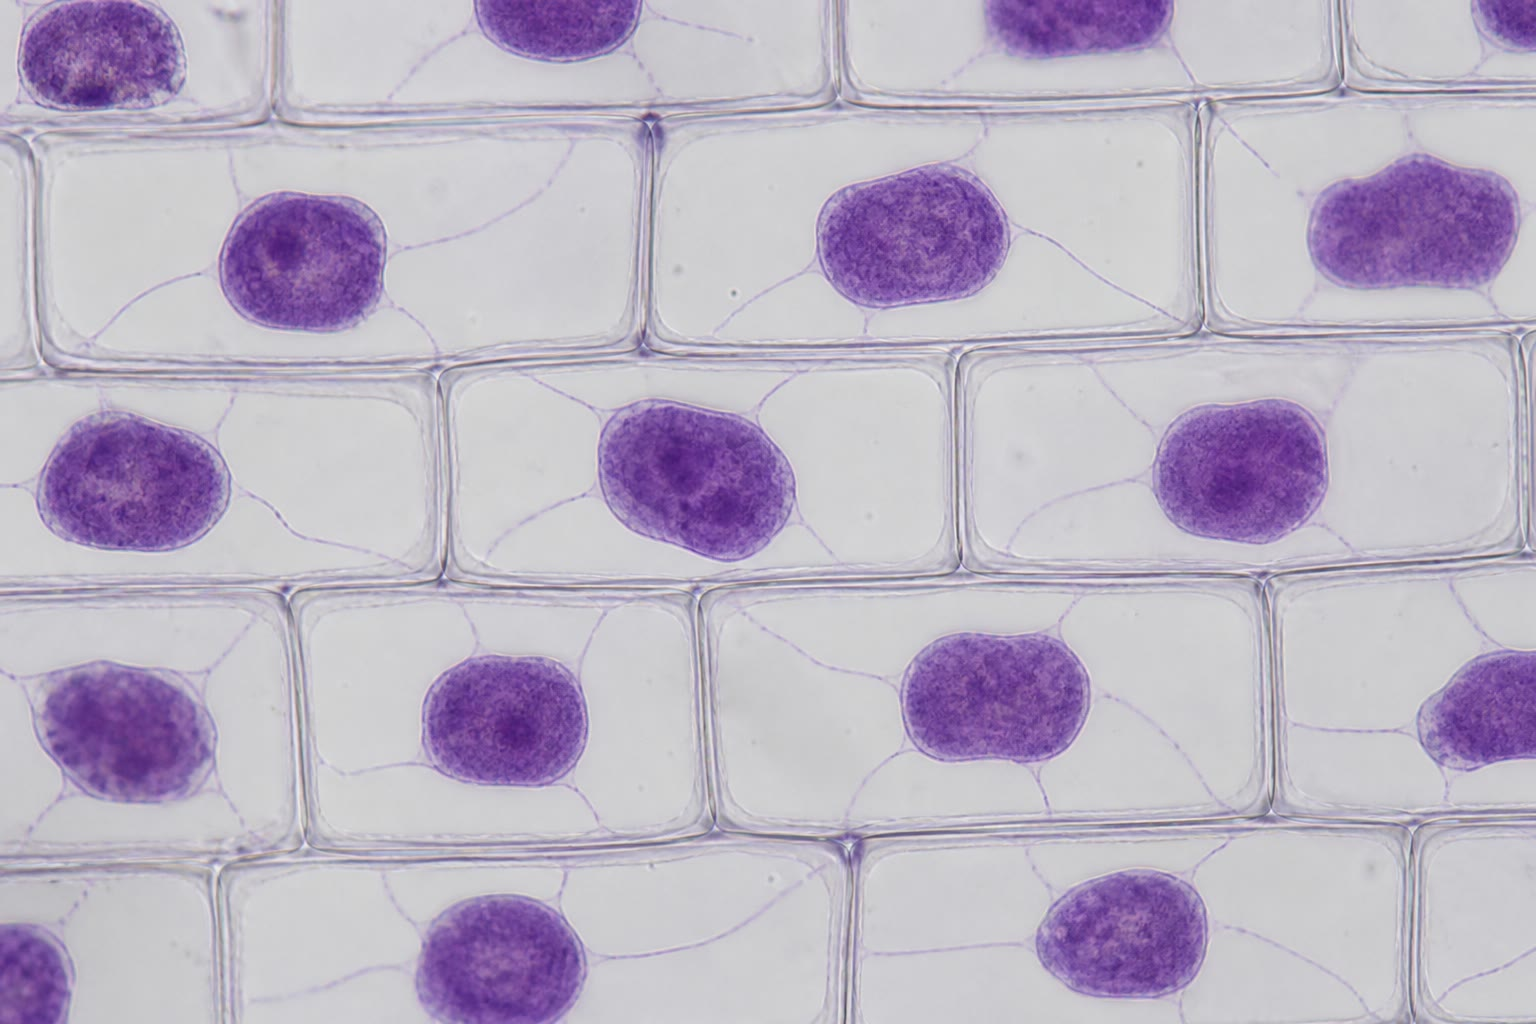
\includegraphics[width=0.6\linewidth]{images/book3/ai/b3-07-plasmolysis.jpg}

{\small La plasmolyse~: épiderme d'oignon dans une solution salée
concentrée. Le protoplaste de chaque \omterm{def:b1:cell-unit-of-life:cell}{cellule} a perdu de l'eau et s'est
décollé de la paroi rigide, qui garde sa forme. Dans l'eau, le
protoplaste regonflerait contre la paroi et s'arrêterait, turgescent.}
\end{omfigure}

\begin{example}[Un globule rouge dans trois solutions]\label{ex:b1:membranes-transport:redcell}
Le \omterm{def:b1:mammal-organization:compartments}{plasma} est à \qty{0.3}{osmol/L}~: $\Psi_s = \qty{-0.74}{MPa}$ des
deux côtés, pas de flux net. Dans l'eau pure ($\Psi = 0$), la \omterm{def:b1:cell-unit-of-life:cell}{cellule},
à \qty{-0.74}{MPa} à l'intérieur, absorbe de l'eau jusqu'à ce que sa
membrane, qui ne peut s'étirer que de quelques pour cent, se rompe. Dans
du sel à \qty{0.6}{osmol/L}, elle perd de l'eau jusqu'à ce que son
intérieur soit aussi concentré, à la moitié de son volume. Une \omterm{def:b1:cell-unit-of-life:cell}{cellule}
végétale dans l'eau pure n'éclate pas~: à mesure que l'eau entre, la
paroi est tendue et $\Psi_p$ monte jusqu'à ce que $\Psi_p = -\Psi_s$, le
\omterm{def:b1:membranes-transport:osmosis}{potentiel hydrique} intérieur est nul, et le flux cesse, la \omterm{def:b1:cell-unit-of-life:cell}{cellule}
restant turgescente à \qty{0.74}{MPa}.
\end{example}

\begin{method}[Faire le bilan des potentiels hydriques]\label{met:b1:membranes-transport:psi}
\begin{enumerate}
  \item Convertir chaque concentration de soluté en osmoles (un sel qui
        se dissocie en deux ions compte double) et calculer $\Psi_s =
        -RTc_s$.
  \item Ajouter le terme de pression~: $\Psi_p = 0$ pour une solution
        dans un récipient ouvert ou pour une \omterm{def:b1:cell-unit-of-life:cell}{cellule} animale, positif
        pour une \omterm{def:b1:cell-unit-of-life:cell}{cellule} végétale turgescente, négatif pour de l'eau
        sous tension dans un vaisseau de \omterm{def:b1:flowering-plant-organization:tissues}{xylème}.
  \item L'eau va vers le $\Psi$ le plus bas. L'équilibre est atteint
        quand les deux $\Psi$ sont égaux~: par dilution du contenu de la
        \omterm{def:b1:cell-unit-of-life:cell}{cellule} (\omterm{def:b1:cell-unit-of-life:cell}{cellule} animale), ou par élévation de la pression
        (\omterm{def:b1:cell-unit-of-life:cell}{cellule} végétale).
  \item Lire le signe du résultat comme le sens du flux, et sa valeur
        comme la force motrice~; le débit dépend aussi de la
        perméabilité de la membrane à l'eau, multipliée par cent par les
        canaux \omterm{def:b1:membranes-transport:transporters}{aquaporines}.
\end{enumerate}
\end{method}

\section{Les protéines de transport}

\begin{definition}[Canaux, transporteurs, pompes]\label{def:b1:membranes-transport:transporters}
Les \emph{canaux}\index{canal} sont des \omterm{def:b1:membranes-transport:proteins}{protéines intrinsèques} munies
d'un pore rempli d'eau par lequel un ion ou une petite molécule
déterminée diffuse selon son gradient, jusqu'à $10^8$ fois par
seconde~; beaucoup sont \emph{à ouverture réglée}, s'ouvrant en réponse
à une tension, à un ligand ou à une force mécanique. Les
\emph{aquaporines}\index{aquaporine} sont des canaux à eau. Les
\emph{transporteurs}\index{transporteur} lient leur soluté sur une face,
changent de conformation, et le libèrent sur l'autre, mille fois par
seconde au plus~; le transporteur du glucose du globule rouge en est un.
Canaux et transporteurs travaillant dans le sens du gradient réalisent
la \emph{diffusion facilitée}\index{diffusion facilitee@diffusion facilitée}, passive mais
sélective et saturable. Les \emph{pompes}\index{pompe} sont des
transporteurs qui couplent le transport d'un soluté contre son gradient
à l'hydrolyse de l'ATP~: le \emph{transport actif
primaire}\index{transport actif}. La \emph{pompe
sodium--potassium}\index{pompe sodium--potassium} des \omterm{def:b1:cell-unit-of-life:cell}{cellules} animales
exporte trois $\mathrm{Na^+}$ et importe deux $\mathrm{K^+}$ par ATP~;
la \emph{pompe à protons} des membranes végétales, fongiques et
bactériennes exporte $\mathrm{H^+}$.
\end{definition}

\begin{omfigure}
\begin{tikzpicture}[font=\footnotesize, >=Stealth, line cap=round]
  % membrane band
  \fill[omDef!15] (0,0) rectangle (13.1,1.2);
  \draw[omDef!60!black] (0,0) -- (13.1,0) (0,1.2) -- (13.1,1.2);
  \node[anchor=east, gray, align=right] at (-0.15,1.5) {extérieur\\ ($\mathrm{Na^+}$ élevé, $\mathrm{K^+}$ bas)};
  \node[anchor=east, gray, align=right] at (-0.15,-0.3) {cytosol\\ ($\mathrm{Na^+}$ bas, $\mathrm{K^+}$ élevé)};
  % simple diffusion
  \draw[->, thick, omProp] (1.0,2.0) -- (1.0,-0.8);
  \node[anchor=south, align=center] at (1.0,2.1) {diffusion simple\\ $\mathrm{O_2}$, $\mathrm{CO_2}$};
  % channel
  \draw[thick, omThm!80!black, fill=omThm!30, rounded corners=2pt] (2.6,-0.2) rectangle (3.0,1.4);
  \draw[thick, omThm!80!black, fill=omThm!30, rounded corners=2pt] (3.3,-0.2) rectangle (3.7,1.4);
  \draw[->, thick, omProp] (3.15,2.0) -- (3.15,-0.8);
  \node[anchor=south, align=center] at (3.15,2.1) {canal\\ $\mathrm{K^+}$, eau};
  % carrier (facilitated)
  \draw[thick, omThm!80!black, fill=omThm!30, rounded corners=5pt] (5.0,-0.3) rectangle (6.0,1.5);
  \draw[->, thick, omProp] (5.5,2.0) -- (5.5,1.55);
  \draw[->, thick, omProp] (5.5,-0.35) -- (5.5,-0.8);
  \node[anchor=south, align=center] at (5.5,2.1) {transporteur\\ glucose};
  \node[align=center, font=\scriptsize] at (5.5,0.6) {lie,\\ bascule};
  % pump
  \draw[thick, omExo!80!black, fill=omExo!30, rounded corners=5pt] (7.5,-0.3) rectangle (8.7,1.5);
  \draw[->, very thick, omExo!80!black] (7.8,-0.8) -- (7.8,2.0);
  \draw[->, very thick, omExo!80!black] (8.4,2.0) -- (8.4,-0.8);
  \node[anchor=south, align=center] at (8.1,2.1) {pompe\\ $3\,\mathrm{Na^+}$ sortent, $2\,\mathrm{K^+}$ entrent};
  \node[anchor=north, align=center, font=\scriptsize] at (8.1,-0.85) {ATP $\to$ ADP};
  % secondary active (symport)
  \draw[thick, omThm!80!black, fill=omThm!30, rounded corners=5pt] (11.0,-0.3) rectangle (12.2,1.5);
  \draw[->, very thick, omProp] (11.3,2.0) -- (11.3,-0.8);
  \draw[->, very thick, omExo!80!black] (11.9,2.0) -- (11.9,-0.8);
  \node[anchor=south, align=center] at (11.6,2.1) {symport\\ $\mathrm{Na^+}$ descend,\\ glucose monte};
  \node[anchor=north, align=center, font=\scriptsize] at (11.6,-0.85) {actif secondaire};
  \node[anchor=north west, align=left, gray, font=\scriptsize] at (0,-1.5) {flèches orange~: sens du gradient (passif)~; vertes~: contre lui (actif)};
\end{tikzpicture}

{\small Cinq façons de traverser. La diffusion simple à travers le
lipide~; un canal et un transporteur (\omterm{def:b1:membranes-transport:transporters}{diffusion facilitée}, dans le sens
du gradient)~; la \omterm{def:b1:membranes-transport:transporters}{pompe sodium--potassium} (\omterm{def:b1:membranes-transport:transporters}{transport actif primaire},
payé en ATP)~; un \omterm{prop:b1:membranes-transport:secondary}{symporteur} qui utilise le gradient de sodium bâti par
la \omterm{def:b1:membranes-transport:transporters}{pompe} pour entraîner le glucose vers le haut (\omterm{prop:b1:membranes-transport:secondary}{transport actif
secondaire}).}
\end{omfigure}

\begin{proposition}[Transport actif secondaire]\label{prop:b1:membranes-transport:secondary}
\index{transport actif secondaire}
Un gradient bâti par une \omterm{def:b1:membranes-transport:transporters}{pompe} est une réserve d'énergie que d'autres
transporteurs dépensent~: un \emph{symporteur}\index{symporteur} fait
monter un soluté contre son gradient en le couplant à un ion qui
descend le sien dans le même sens (le transporteur sodium--glucose de
l'intestin et du rein~; le transporteur proton--saccharose du phloème),
un \emph{antiporteur}\index{antiporteur} le couple à un ion qui se
déplace en sens inverse (l'échangeur sodium--calcium). Dans les \omterm{def:b1:cell-unit-of-life:cell}{cellules}
animales la monnaie est le gradient de $\mathrm{Na^+}$~; chez les
végétaux, les champignons et les bactéries, le gradient de
$\mathrm{H^+}$.
\end{proposition}

\begin{example}[La cinétique révèle le mécanisme]\label{ex:b1:membranes-transport:kinetics}
Le flux de glucose entrant dans un globule rouge croît avec la
concentration extérieure, puis plafonne à un maximum, comme pour une
enzyme (\cref{ch:b1:enzymes})~: un transporteur, saturable, de $K_m$
voisin de \qty{1.5}{mmol/L}~; un sucre voisin, le mannose, entre en
compétition avec lui. Le flux d'urée croît proportionnellement à sa
concentration sans limite~: diffusion simple. Le flux de glucose entrant
dans une \omterm{def:b1:cell-unit-of-life:cell}{cellule} intestinale cesse si l'on retire le sodium de la
lumière, ou si l'on empoisonne la \omterm{def:b1:membranes-transport:transporters}{pompe} à l'ouabaïne~: \omterm{prop:b1:membranes-transport:secondary}{transport actif
secondaire}.
\end{example}

\section{Le potentiel de membrane}

\begin{definition}[Potentiel de membrane]\label{def:b1:membranes-transport:potential}
Toute \omterm{def:b1:cell-unit-of-life:cell}{cellule} vivante maintient une différence de potentiel électrique
de part et d'autre de sa \omterm{def:b1:membranes-transport:membrane}{membrane plasmique}, le \emph{potentiel de
membrane}\index{potentiel de membrane} $V_m = V_{\text{int}} - V_{\text{ext}}$, négatif à l'intérieur~:
\qty{-70}{mV} dans un \omterm{def:b1:body-plans-tissues:nervous}{neurone}, \qty{-90}{mV} dans une fibre musculaire,
\qty{-120}{mV} ou davantage dans une \omterm{def:b1:cell-unit-of-life:cell}{cellule} végétale. Il provient de ce
que la membrane est sélectivement perméable à des ions dont les
concentrations diffèrent de part et d'autre.
\end{definition}

\begin{theorem}[L'équation de Nernst]\label{thm:b1:membranes-transport:nernst}
\index{equation de Nernst@équation de Nernst}\index{potentiel d'equilibre@potentiel d'équilibre}
Un ion de charge $z$ aux concentrations $c_{\text{ext}}$ et
$c_{\text{int}}$ est à l'équilibre de part et d'autre de la membrane ---
aucun flux net, bien que la membrane lui soit perméable --- lorsque le
potentiel égale son \emph{\omterm{thm:b1:membranes-transport:nernst}{potentiel d'équilibre}}
\[
E_{\text{ion}} = \frac{RT}{zF}\,\ln\frac{c_{\text{ext}}}{c_{\text{int}}}
= \frac{\qty{61.5}{mV}}{z}\,\log_{10}\frac{c_{\text{ext}}}{c_{\text{int}}}
\quad (\qty{37}{\celsius}).
\]
Pour $\mathrm{K^+}$ à \qty{5}{mmol/L} au-dehors et \qty{140}{mmol/L}
au-dedans, $E_K = 61.5\log(5/140) = \qty{-89}{mV}$~; pour
$\mathrm{Na^+}$ à \qty{145}{} au-dehors et \qty{12}{} au-dedans,
$E_{Na} = \qty{+67}{mV}$.
\end{theorem}
\begin{proof}
Faire passer une mole de l'ion du dehors au dedans change l'énergie
libre de la somme d'un terme de concentration et d'un terme
électrique~:
\[
\Delta G = RT\ln\frac{c_{\text{int}}}{c_{\text{ext}}} + zFV_m .
\]
À l'équilibre $\Delta G = 0$, ce qui donne $V_m = (RT/zF)\ln(c_{\text{ext}}/c_{\text{int}})$.
Le passage aux logarithmes décimaux et l'introduction de $R = \qty{8.314}{J.mol^{-1}.K^{-1}}$,
$T = \qty{310}{K}$, $F = \qty{96485}{C/mol}$ donnent la forme numérique.
\end{proof}

\begin{proposition}[Origine du potentiel de repos]\label{prop:b1:membranes-transport:resting}
La membrane au repos est bien plus perméable à $\mathrm{K^+}$ (par des
canaux potassiques ouverts) qu'à $\mathrm{Na^+}$~; $\mathrm{K^+}$ fuit
vers l'extérieur selon son gradient de concentration, laissant
l'intérieur négatif, jusqu'à ce que l'attraction électrique en retour
équilibre presque la fuite. Le potentiel de repos est donc voisin de
$E_K$, tiré un peu vers $E_{Na}$ par la faible fuite de sodium
(l'équation de Goldman pondère le terme de Nernst de chaque ion par sa
perméabilité). La \omterm{def:b1:membranes-transport:transporters}{pompe} entretient les gradients que les fuites
dissiperaient sinon~; elle contribue aussi de quelques millivolts
directement, puisqu'elle sort trois charges pour deux qui entrent.
\end{proposition}
\begin{proof}[Faits expérimentaux]
Dans un axone géant de calmar, le potentiel de repos suit $E_K$ quand on
fait varier le potassium extérieur sur un large domaine (une droite de
pente \qty{58}{mV} par décade aux fortes concentrations), et s'en écarte
aux faibles concentrations exactement comme le prévoit une faible
perméabilité au sodium. Bloquer la \omterm{def:b1:membranes-transport:transporters}{pompe} à l'ouabaïne laisse le
potentiel presque inchangé pendant quelques minutes, puis le laisse
décroître en quelques heures à mesure que les gradients s'épuisent~: le
potentiel est un potentiel de diffusion, la \omterm{def:b1:membranes-transport:transporters}{pompe} en est le soutien à
long terme.
\end{proof}

\begin{omfigure}
\begin{tikzpicture}
\begin{semilogxaxis}[
  width=0.86\linewidth, height=6.2cm,
  axis x line=bottom, axis y line=left,
  xmin=0.8, xmax=200, ymin=-135, ymax=10,
  xlabel={$\mathrm{K^+}$ extérieur (\unit{mmol/L})}, ylabel={potentiel de membrane (\unit{mV})},
  xlabel style={font=\small, at={(axis description cs:0.5,-0.12)}, anchor=north},
  ylabel style={font=\small},
  tick label style={font=\small}, xtick={1,10,100}, log ticks with fixed point, ytick={-120,-100,-80,-60,-40,-20,0},
  legend style={font=\small, at={(0.03,0.97)}, anchor=north west, draw=none},
  clip=false,
]
\addplot[thick, dashed, omDef, domain=0.8:200, samples=40] {58*log10(x/140)};
\addlegendentry{Nernst $E_K$ (pente \qty{58}{mV} par décade)}
\addplot[very thick, omThm, domain=0.8:200, samples=60] {58*log10((x+0.01*145)/(140+0.01*12))};
\addlegendentry{mesuré~: $\mathrm{K^+}$ plus une faible fuite de $\mathrm{Na^+}$}
\draw[dashed, gray] (axis cs:5,-135) -- (axis cs:5,-82);
\node[font=\scriptsize, anchor=west] at (axis cs:5.5,-120) {physiologique~: \qty{5}{mmol/L}};
\end{semilogxaxis}
\end{tikzpicture}

{\small Potentiel de repos en fonction du potassium extérieur. Aux
fortes concentrations, la membrane se comporte comme une électrode à
potassium et suit la droite de Nernst~; aux faibles concentrations, la
faible fuite de sodium le tire au-dessus de $E_K$.}
\end{omfigure}

\begin{example}[Où passe l'énergie de la pompe]\label{ex:b1:membranes-transport:pumpcost}
Sortir un $\mathrm{Na^+}$ contre un gradient de \qty{12}{} à
\qty{145}{mmol/L} et \qty{-70}{mV} coûte
$RT\ln(145/12) + F\times 0.070 = 6.4 + 6.8 =
\qty{13.2}{kJ/mol}$~; trois d'entre eux, \qty{40}{kJ}, plus deux
$\mathrm{K^+}$ entrants à $RT\ln(140/5) - F\times 0.070 = 8.6 - 6.8 =
\qty{1.8}{kJ/mol}$ chacun~: \qty{43}{kJ} par cycle contre les
\qty{50}{kJ} d'un ATP dans les conditions cellulaires. La \omterm{def:b1:membranes-transport:transporters}{pompe}
fonctionne près de sa limite thermodynamique, et elle consomme le tiers
de l'ATP d'un animal au repos, les deux tiers dans l'encéphale.
\end{example}

\section{Le transport en masse}

\begin{proposition}[Transport vésiculaire]\label{prop:b1:membranes-transport:vesicles}
Macromolécules et particules franchissent la \omterm{def:b1:membranes-transport:membrane}{membrane plasmique} sans la
traverser~: par \emph{exocytose}, une vésicule fusionne avec la membrane
et se vide vers l'extérieur~; par \emph{\omterm{def:b1:eukaryotic-cell:endocytosis}{endocytose}}, la membrane englobe
du matériel dans une vésicule (\cref{ch:b1:eukaryotic-cell}). Les deux
exigent de l'ATP, les deux déplacent de la membrane autant que du
contenu, et les deux conservent l'orientation de la membrane. Les trois
voies de franchissement d'une membrane --- à travers le lipide, à
travers une protéine, à l'intérieur d'une vésicule --- sont sélectives
de trois façons~: par la solubilité, par la reconnaissance moléculaire,
par le choix de ce qui est englobé.
\end{proposition}

\begin{example}[La livraison du cholestérol]\label{ex:b1:membranes-transport:ldl}
Le cholestérol voyage dans le sang à l'intérieur de particules
enveloppées de protéines, trop grosses pour un quelconque transporteur.
Une \omterm{def:b1:cell-unit-of-life:cell}{cellule} qui a besoin de cholestérol expose des récepteurs de la
particule~; particule et récepteur se rassemblent dans un puits
recouvert, qui s'étrangle, et la vésicule livre la particule à un
\omterm{def:b1:eukaryotic-cell:endomembrane}{lysosome} où le cholestérol est libéré. Une personne dont les récepteurs
sont défectueux ne peut pas épurer les particules~: le cholestérol
sanguin double et les artères s'obstruent dès le début de l'âge adulte.
Une \omterm{def:b1:membranes-transport:membrane}{protéine membranaire}, une maladie.
\end{example}

\section{Exercices}

\begin{exercise}[$\star$]\label{exo:b1:membranes-transport:1}
Décrire le \omterm{def:b1:membranes-transport:membrane}{modèle de la mosaïque fluide} en quatre phrases~: les lipides,
les protéines, la fluidité, l'asymétrie.
\end{exercise}

\begin{exercise}[$\star$]\label{exo:b1:membranes-transport:2}
Classer $\mathrm{O_2}$, le glucose, $\mathrm{Na^+}$, l'eau et l'éthanol
selon leur perméabilité à travers une \omterm{def:b1:membranes-transport:membrane}{bicouche lipidique} pure, et
expliquer cet ordre.
\end{exercise}

\begin{exercise}[$\star$]\label{exo:b1:membranes-transport:3}
Calculer le \omterm{def:b1:membranes-transport:osmosis}{potentiel osmotique} d'une solution de saccharose à
\qty{0.1}{mol/L} et d'une solution de NaCl à \qty{0.1}{mol/L}, à
\qty{25}{\celsius}.
\end{exercise}

\begin{exercise}[$\star$]\label{exo:b1:membranes-transport:4}
Calculer le potentiel de Nernst de $\mathrm{Cl^-}$ à \qty{120}{mmol/L}
au-dehors et \qty{4}{mmol/L} au-dedans, à \qty{37}{\celsius}. Le
chlorure est-il à l'équilibre dans une \omterm{def:b1:cell-unit-of-life:cell}{cellule} à \qty{-89}{mV}~?
\end{exercise}

\begin{exercise}[$\star\star$]\label{exo:b1:membranes-transport:5}
Gorter et Grendel employèrent $\num{4.7e9}$ globules rouges de
\qty{100}{\micro m^2} de surface chacun et obtinrent une monocouche
lipidique de \qty{0.92}{m^2}. Calculer le rapport de l'aire de la
monocouche à la surface cellulaire et conclure.
\end{exercise}

\begin{exercise}[$\star\star$]\label{exo:b1:membranes-transport:6}
Une \omterm{def:b1:cell-unit-of-life:cell}{cellule} végétale a un \omterm{def:b1:membranes-transport:osmosis}{potentiel osmotique} de \qty{-0.9}{MPa} et un
\omterm{def:b1:membranes-transport:osmosis}{potentiel de pression} de \qty{0.5}{MPa}. On la place dans une solution
de \omterm{def:b1:membranes-transport:osmosis}{potentiel osmotique} \qty{-0.6}{MPa}, dans un récipient ouvert. Dans
quel sens l'eau se déplace-t-elle, et quel est le \omterm{def:b1:membranes-transport:osmosis}{potentiel de pression}
de la \omterm{def:b1:cell-unit-of-life:cell}{cellule} à l'équilibre (on supposera son \omterm{def:b1:membranes-transport:osmosis}{potentiel osmotique}
inchangé)~?
\end{exercise}

\begin{exercise}[$\star\star$]\label{exo:b1:membranes-transport:7}
L'absorption de glucose par une \omterm{def:b1:cell-unit-of-life:cell}{cellule} est mesurée à des
concentrations extérieures croissantes~: \qtylist{1;2;5;10;20}{mmol/L}
donnent \qtylist{0.4;0.67;1.0;1.25;1.43}{\micro mol/min}. Montrer que
l'absorption sature, estimer la vitesse maximale et la concentration
qui en donne la moitié, et nommer le mécanisme.
\end{exercise}

\begin{exercise}[$\star\star$]\label{exo:b1:membranes-transport:8}
Expliquer pourquoi le potentiel de repos d'une \omterm{def:b1:cell-unit-of-life:cell}{cellule} est voisin de
$E_K$ et non de $E_{Na}$, et ce qui lui arriverait si des canaux
sodiques s'ouvraient brusquement.
\end{exercise}

\begin{exercise}[$\star\star$]\label{exo:b1:membranes-transport:9}
Le \omterm{prop:b1:membranes-transport:secondary}{symporteur} sodium--glucose transporte deux $\mathrm{Na^+}$ par
glucose. Avec $\mathrm{Na^+}$ à \qty{145}{mmol/L} au-dehors et
\qty{12}{} au-dedans et $V_m = \qty{-60}{mV}$, calculer l'énergie libre
disponible dans les deux ions sodium et le rapport maximal de
concentrations de glucose (intérieur/extérieur) que le \omterm{prop:b1:membranes-transport:secondary}{symporteur} peut
établir à \qty{37}{\celsius}.
\end{exercise}

\begin{exercise}[$\star\star\star$]\label{exo:b1:membranes-transport:10}
Une \omterm{def:b1:cell-unit-of-life:cell}{cellule} est refroidie à \qty{4}{\celsius}. Prédire, en justifiant,
les effets sur~: la fluidité membranaire, la diffusion simple de
$\mathrm{O_2}$, la \omterm{def:b1:membranes-transport:transporters}{pompe}, les gradients ioniques au bout de quelques
heures, le \omterm{def:b1:membranes-transport:potential}{potentiel de membrane}, et le volume de la \omterm{def:b1:cell-unit-of-life:cell}{cellule}. (On
considérera que les protéines de la \omterm{def:b1:cell-unit-of-life:cell}{cellule} exercent une attraction
osmotique que le gradient de sodium équilibre normalement.)
\end{exercise}

\begin{exercise}[$\star\star\star$]\label{exo:b1:membranes-transport:11}
Les \omterm{def:b1:cell-unit-of-life:cell}{cellules} fusionnées de Frye et Edidin montrèrent un mélange complet
des protéines de surface à \qty{37}{\celsius} en \qty{40}{min}, aucun à
\qty{4}{\celsius}, et aucun à \qty{37}{\celsius} lorsque la synthèse
d'ATP était bloquée --- ce dernier résultat s'est révélé faux par la
suite. Dire ce que chaque résultat impliquerait sur le mécanisme du
mélange, et pourquoi la version correcte (le mélange n'a pas besoin
d'ATP) importe pour le \omterm{def:b1:membranes-transport:membrane}{modèle de la mosaïque fluide}.
\end{exercise}

\begin{exercise}[$\star\star\star$]\label{exo:b1:membranes-transport:12}
«~Le \omterm{def:b1:membranes-transport:potential}{potentiel de membrane} est un sous-produit des gradients ioniques,
et non quelque chose que la \omterm{def:b1:cell-unit-of-life:cell}{cellule} bâtit directement.~» Discuter en un
paragraphe, à l'aide de l'\omterm{thm:b1:membranes-transport:nernst}{équation de Nernst}, de la \omterm{def:b1:membranes-transport:transporters}{pompe}, et du nombre
d'ions réellement nécessaire pour charger la membrane (capacité de
\qty{1}{\micro F/cm^2}).
\end{exercise}

\section{Problème~: l'entérocyte}

\begin{problem}[{Problème du week-end --- la cellule qui extrait le
glucose de l'intestin~: pompe, symporteur, transporteur et équation de
Nernst, jusqu'au plus grand rapport de glucose que la cellule peut
établir}]
\label{pb:b1:membranes-transport:1}
Une \omterm{def:b1:cell-unit-of-life:cell}{cellule} épithéliale intestinale (entérocyte) est haute de
\qty{25}{\micro m} et large de \qty{5}{\micro m}~; sa membrane apicale
donne sur la lumière, sa membrane basolatérale sur le sang. Son \omterm{def:b1:eukaryotic-cell:organelle}{cytosol}
contient \qty{12}{mmol/L} de $\mathrm{Na^+}$ et \qty{140}{mmol/L} de
$\mathrm{K^+}$~; la lumière et le sang contiennent \qty{145}{mmol/L} de
$\mathrm{Na^+}$ et \qty{5}{mmol/L} de $\mathrm{K^+}$. Le \omterm{def:b1:membranes-transport:potential}{potentiel de
membrane} vaut \qty{-60}{mV}. Prendre $T = \qty{310}{K}$,
$R = \qty{8.314}{J.mol^{-1}.K^{-1}}$, $F = \qty{96500}{C/mol}$,
$RT/F = \qty{26.7}{mV}$, et
$\Delta G_{\text{ATP}} = \qty{-50}{kJ/mol}$ dans la \omterm{def:b1:cell-unit-of-life:cell}{cellule}.

\medskip
\noindent\textbf{Partie I --- Les gradients.}
\begin{enumerate}
  \item Calculer les potentiels de Nernst de $\mathrm{Na^+}$ et de
        $\mathrm{K^+}$.
  \item Quel ion est le plus proche de l'équilibre à \qty{-60}{mV}~? Que
        dit cela des perméabilités au repos~?
  \item Calculer la variation d'énergie libre pour une mole de
        $\mathrm{Na^+}$ entrant dans la \omterm{def:b1:cell-unit-of-life:cell}{cellule}, et pour une mole de
        $\mathrm{K^+}$ en sortant.
  \item Calculer le coût en énergie libre d'un cycle de \omterm{def:b1:membranes-transport:transporters}{pompe}
        ($3\,\mathrm{Na^+}$ sortants, $2\,\mathrm{K^+}$ entrants) et le
        comparer à l'énergie d'un ATP. Quel est le rendement~?
  \item La \omterm{def:b1:membranes-transport:transporters}{pompe} n'est présente que sur la membrane basolatérale.
        Expliquer pourquoi cette localisation est nécessaire pour que la
        \omterm{def:b1:cell-unit-of-life:cell}{cellule} déplace le glucose de la lumière vers le sang.
\end{enumerate}

\medskip
\noindent\textbf{Partie II --- Le glucose contre le gradient.}
La membrane apicale porte un \omterm{prop:b1:membranes-transport:secondary}{symporteur} qui fait entrer un glucose avec
deux $\mathrm{Na^+}$~; la membrane basolatérale porte un transporteur du
glucose (\omterm{def:b1:membranes-transport:transporters}{diffusion facilitée}).
\begin{enumerate}[resume]
  \item Calculer l'énergie libre libérée par deux $\mathrm{Na^+}$
        entrant dans la \omterm{def:b1:cell-unit-of-life:cell}{cellule}.
  \item Écrire l'énergie libre nécessaire pour faire passer un glucose
        de la lumière (concentration $c_L$) au \omterm{def:b1:eukaryotic-cell:organelle}{cytosol} ($c_C$).
  \item À la limite du \omterm{prop:b1:membranes-transport:secondary}{symporteur}, les deux sont égales. Calculer le
        rapport maximal $c_C/c_L$.
  \item Si la lumière tombe à \qty{0.1}{mmol/L} de glucose en fin
        d'absorption, quelle concentration cytosolique le \omterm{prop:b1:membranes-transport:secondary}{symporteur}
        peut-il encore maintenir~?
  \item La glycémie vaut \qty{5}{mmol/L}. Expliquer comment le glucose
        quitte la \omterm{def:b1:cell-unit-of-life:cell}{cellule} vers le sang sans énergie supplémentaire.
  \item Pourquoi le \omterm{prop:b1:membranes-transport:secondary}{symporteur} est-il placé sur la membrane apicale et
        le transporteur sur la basolatérale, et non l'inverse~?
  \item Les solutions de réhydratation orale contre le choléra
        contiennent du glucose et du sel. Expliquer, à partir du
        \omterm{prop:b1:membranes-transport:secondary}{symporteur}, pourquoi le glucose fait absorber le sel --- et
        l'eau.
\end{enumerate}

\medskip
\noindent\textbf{Partie III --- Compter le trafic.}
La \omterm{def:b1:cell-unit-of-life:cell}{cellule} absorbe \qty{2e-15}{mol} de glucose par seconde.
\begin{enumerate}[resume]
  \item Calculer le $\mathrm{Na^+}$ qui entre par seconde par les
        \omterm{prop:b1:membranes-transport:secondary}{symporteurs}, et le nombre de cycles de \omterm{def:b1:membranes-transport:transporters}{pompe} par seconde
        nécessaires pour l'exporter.
  \item Calculer l'ATP dépensé par seconde pour cette exportation, et la
        fraction du glucose absorbé qu'il faudrait respirer pour la
        payer (environ 30 ATP par glucose).
  \item Chaque \omterm{prop:b1:membranes-transport:secondary}{symporteur} effectue \qty{50}{} cycles par seconde.
        Combien de \omterm{prop:b1:membranes-transport:secondary}{symporteurs} la membrane apicale doit-elle porter~? La
        membrane apicale fait \qty{25}{\micro m^2}, multipliée par
        \qty{20}{} par les microvillosités~: calculer la densité de
        \omterm{prop:b1:membranes-transport:secondary}{symporteurs} par micromètre carré.
  \item Le $\mathrm{Na^+}$ qui entre appelle de l'eau par \omterm{def:b1:membranes-transport:osmosis}{osmose}. Deux
        $\mathrm{Na^+}$ et un glucose, avec le $\mathrm{Cl^-}$
        accompagnateur, font quatre osmoles~; la \omterm{def:b1:cell-unit-of-life:cell}{cellule} maintient son
        osmolarité à \qty{0.3}{osmol/L}. Calculer le volume d'eau qui
        doit suivre les solutés par seconde, et le temps qu'il faudrait
        pour doubler le volume de la \omterm{def:b1:cell-unit-of-life:cell}{cellule} si l'eau ne sortait pas par
        la membrane basolatérale.
  \item Calculer le nombre de molécules d'eau absorbées par molécule de
        glucose (\qty{18}{g/mol}, masse volumique \qty{1}{g/mL}).
\end{enumerate}

\medskip
\noindent\textbf{Partie IV --- Charger la membrane.}
La membrane est un condensateur de \qty{1}{\micro F/cm^2}.
\begin{enumerate}[resume]
  \item Calculer l'aire de la membrane de la \omterm{def:b1:cell-unit-of-life:cell}{cellule} (prendre un pavé de
        \qty{25}{\micro m} sur \qty{5}{\micro m} sur \qty{5}{\micro m}
        sans microvillosités) et sa capacité.
  \item Calculer la charge nécessaire pour maintenir \qty{-60}{mV} et le
        nombre d'ions monovalents qu'elle représente.
  \item Calculer le nombre d'ions en excès par micromètre carré de
        membrane que cela représente.
  \item Calculer le nombre d'ions $\mathrm{K^+}$ de la \omterm{def:b1:cell-unit-of-life:cell}{cellule}, et la
        fraction qui doit sortir pour charger la membrane. Commenter.
  \item La \omterm{def:b1:membranes-transport:transporters}{pompe} sort une charge nette à chaque cycle. À l'aide de la
        question 13, calculer le courant qu'elle porte et la variation
        de potentiel qu'elle produirait en une seconde si rien d'autre
        ne bougeait. Pourquoi le potentiel ne s'emballe-t-il pas en
        réalité~?
  \item Une substance bloque la \omterm{def:b1:membranes-transport:transporters}{pompe}. Prédire, dans l'ordre, les
        changements du gradient de sodium, de l'absorption du glucose,
        du \omterm{def:b1:membranes-transport:potential}{potentiel de membrane} et du volume cellulaire.
  \item Une substance bloque au contraire les canaux potassiques.
        Prédire la variation du potentiel de repos.
  \item Énoncer le résultat~: le rapport maximal de concentrations de
        glucose que l'entérocyte peut établir, et les deux \omterm{def:b1:membranes-transport:membrane}{protéines
        membranaires} qui le rendent possible.
\end{enumerate}
\end{problem}
